\documentclass[10pt,twocolumn,letterpaper]{article}

\usepackage[pagenumbers]{cvpr}
\usepackage{graphicx}
\usepackage{amsmath}
\usepackage{amssymb}
\usepackage{booktabs}
\usepackage[utf8]{inputenc}
\usepackage{graphicx}
\usepackage{scalefnt}
\usepackage{textfit}
\usepackage{float}
\usepackage{cite}
\usepackage{stmaryrd}
\usepackage[linesnumbered,lined,boxed,ruled,commentsnumbered]{algorithm2e}
\usepackage{bm}
\usepackage{textcomp}
\usepackage{amsfonts}
\usepackage[acronym]{glossaries}
\usepackage[pagebackref,breaklinks,colorlinks]{hyperref}
\usepackage[capitalize]{cleveref}
\crefname{section}{Sec.}{Secs.}
\Crefname{section}{Section}{Sections}
\Crefname{table}{Table}{Tables}
\crefname{table}{Tab.}{Tabs.}

\usepackage{etoolbox}
\renewcommand{\thesection}{\Roman{section}}
\renewcommand{\thesubsection}{\thesection.\arabic{subsection}}

\SetKwComment{Comment}{\%\% }{ \%\%}
\SetKwInput{KwInput}{Input}
\SetKwInput{KwOutput}{Output}


\begin{document}

\title{Machine Learning for Time Series \\ \textit{Time warp invariant kSVD:\\ Sparse coding and dictionary learning for time series under time warp}}

\author{Manal Akhannouss, ENS Paris-Saclay\\
{\tt\small manal.akhannouss@eleves.enpc.fr}
\and
Alexandre Lutt, ENS Paris-Saclay\\
{\tt\small alexandre.lutt@eleves.enpc.fr}
}
\maketitle


\section{Introduction}
\label{sec:intro}

\paragraph{} We're gonna talk about \cite{main_paper}.


\section{Models}
\label{sec:models}

\subsection{Sparse coding}

\subsubsection{Orthogonal Matching Pursuit}

\paragraph{} 

\subsubsection{TWI Orthogonal Matching Pursuit}

\paragraph{} 

\subsection{Dictionnary learning}

\subsubsection{k-SVD}

\paragraph{} 

\subsubsection{TWI k-SVD}

\paragraph{} 


\section{Experimental setup}
\label{sec:setup}

\subsection{BME Dataset}

\paragraph{} 

\subsection{DIGITS Dataset}

\paragraph{} 

\subsection{Evaluation metrics}

\paragraph{} 


\section{Results}
\label{sec:results}

\subsection{BME dataset}

\paragraph{} 

\subsection{DIGITS dataset}

\paragraph{} 


\section{Conclusion}
\label{sec:conclusion}

\paragraph{} 

\section{Appendix}
\label{sec:appendix}

\begin{table*}[ht]
    \centering
        \begin{tabular}{ccc}
            \toprule
            \textbf{Sparsity/Models} & \textbf{kSVD} & \textbf{TWI-kSVD} \\
            \midrule
            \textbf{2} & $0.25889$ & $0.17313$ \\
            \textbf{5} & $0.19553$ & $0.12301$ \\
            \textbf{10} & $0.14806$ & $\bm{0.08559}$ \\
            \bottomrule
        \end{tabular}
    \caption{Reconstruction $L_2$ errors on the BME dataset (lower is better)}
    \label{tab:reconstruction_results_BME}
\end{table*}

\begin{table*}[!ht]
    \begin{minipage}{.55\linewidth}
      \centering
        \begin{tabular}{ccc}
            \toprule
            \textbf{Sparsity/Models} & \textbf{kSVD} & \textbf{TWI-kSVD} \\
            \midrule
            \textbf{2} & $\bm{0.20}$ & $0.58$ \\
            \textbf{5} & $0.30$ & $0.58$ \\
            \textbf{10} & $0.42$ & $0.47$ \\
            \bottomrule
        \end{tabular}
        \caption{Original classification strategy}
    \end{minipage}
    \begin{minipage}{.35\linewidth}
      \centering
        \begin{tabular}{ccc}
            \toprule
            \textbf{Sparsity/Models} & \textbf{kSVD} & \textbf{TWI-kSVD} \\
            \midrule
            \textbf{2} & $\bm{0.12}$ & $0.53$ \\
            \textbf{5} & $\bm{0.12}$ & $0.53$ \\
            \textbf{10} & $0.18$ & $0.62$ \\
            \bottomrule
        \end{tabular}
        \caption{Our classification strategy}
    \end{minipage} 
    \caption{Classification error rates on the BME dataset (lower is better)}
    \label{tab:classif_results_BME}
\end{table*}

\begin{table*}[ht]
    \centering
        \begin{tabular}{ccc}
            \toprule
            \textbf{Sparsity/Models} & \textbf{kSVD} & \textbf{TWI-kSVD} \\
            \midrule
            \textbf{2} & $0.50032$ & $0.53786$ \\
            \textbf{5} & $0.30314$ & $0.32883$ \\
            \textbf{10} & $\bm{0.20322}$ & $0.21764$ \\
            \bottomrule
        \end{tabular}
    \caption{Reconstruction $L_2$ errors on the DIGITS dataset (lower is better)}
    \label{tab:reconstruction_results_DIGITS}
\end{table*}

\begin{table*}[!ht]
    \begin{minipage}{.55\linewidth}
      \centering
        \begin{tabular}{ccc}
            \toprule
            \textbf{Sparsity/Models} & \textbf{kSVD} & \textbf{TWI-kSVD} \\
            \midrule
            \textbf{2} & $\bm{0.26}$ & $0.73$ \\
            \textbf{5} & $0.50$ & $0.66$ \\
            \textbf{10} & $0.65$ & $0.92$ \\
            \bottomrule
        \end{tabular}
        \caption{Original classification strategy}
    \end{minipage}
    \begin{minipage}{.35\linewidth}
      \centering
        \begin{tabular}{ccc}
            \toprule
            \textbf{Sparsity/Models} & \textbf{kSVD} & \textbf{TWI-kSVD} \\
            \midrule
            \textbf{2} & $\bm{0.14}$ & $0.81$ \\
            \textbf{5} & $0.24$ & $0.76$ \\
            \textbf{10} & $0.30$ & $0.88$ \\
            \bottomrule
        \end{tabular}
        \caption{Our classification strategy}
    \end{minipage} 
    \caption{Classification error rates on the DIGITS dataset (lower is better)}
    \label{tab:classif_results_DIGITS}
\end{table*}

\begin{figure*}
    \centering
    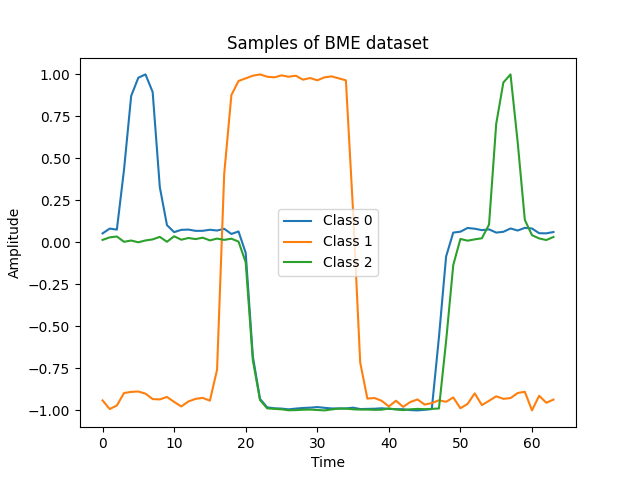
\includegraphics[scale=0.7]{../../figures/BME_samples.png}
    \caption{Samples of each class of the BME dataset} \label{fig:BME_samples}
\end{figure*}


\begin{figure*}
    \centering
    \begin{subfigure}[b]{0.49\textwidth}
      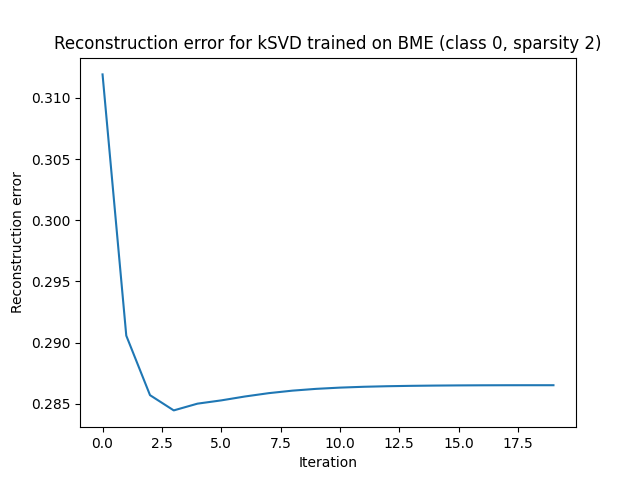
\includegraphics[width=\textwidth]{../../figures/loss_kSVD_spars_2_class_0_BME.png}
      \caption{kSVD}
    \end{subfigure}
    \begin{subfigure}[b]{0.49\textwidth}
        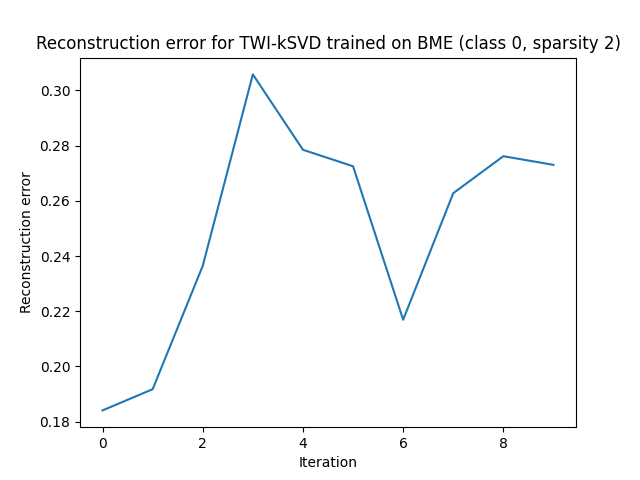
\includegraphics[width=\textwidth]{../../figures/loss_TWI_kSVD_spars_2_class_0_BME.png}
        \caption{TWI-kSVD}
      \end{subfigure}

    \caption{Evolution of reconstruction loss during training (BME dataset)}\label{fig:loss_BME}
\end{figure*}

\begin{figure*}
    \centering
    \begin{subfigure}[t]{\textwidth}
        \centering
        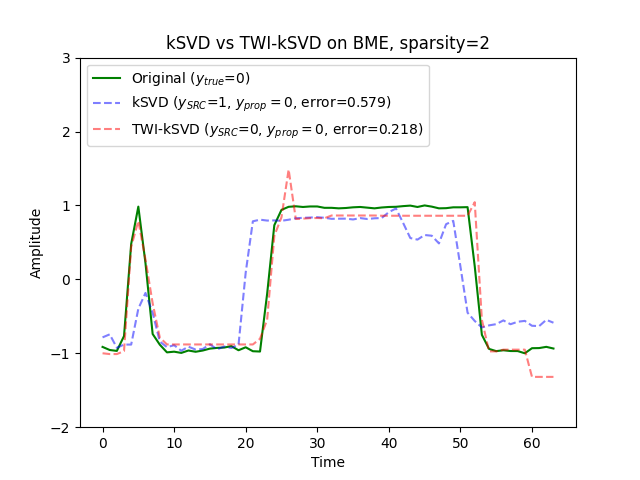
\includegraphics[scale=0.6]{../../figures/1D_example_sparsity_2.png}
        \caption{Sparsity = 2}
    \end{subfigure}
    
    \begin{subfigure}[t]{\textwidth}
        \centering
        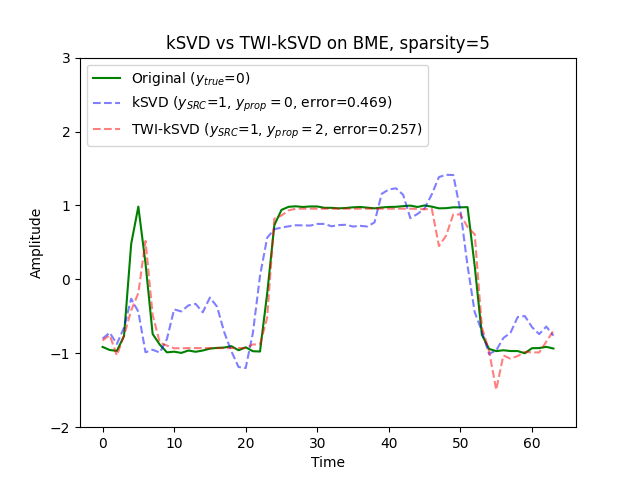
\includegraphics[scale=0.6]{../../figures/1D_example_sparsity_5.png}
        \caption{Sparsity = 5}
    \end{subfigure}

    \begin{subfigure}[t]{\textwidth}
        \centering
        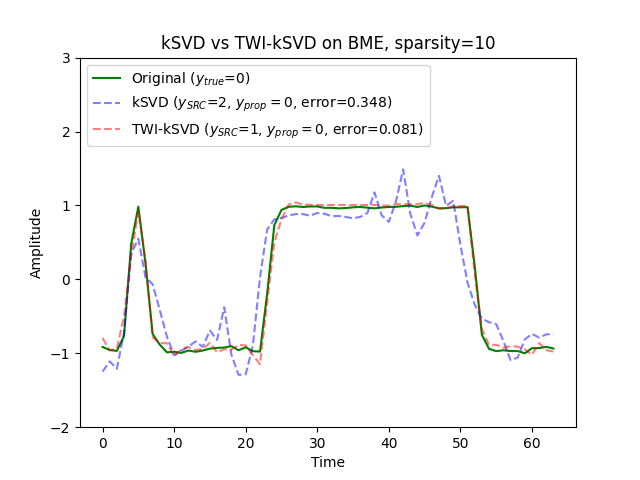
\includegraphics[scale=0.6]{../../figures/1D_example_sparsity_10.png}
        \caption{Sparsity = 10}
    \end{subfigure}
        \caption{Example of reconstructions (BME dataset) with different sparsity levels}\label{tab:1D_example}
\end{figure*}

\begin{figure*}
    \centering
    \begin{subfigure}[t]{\textwidth}
        \centering
        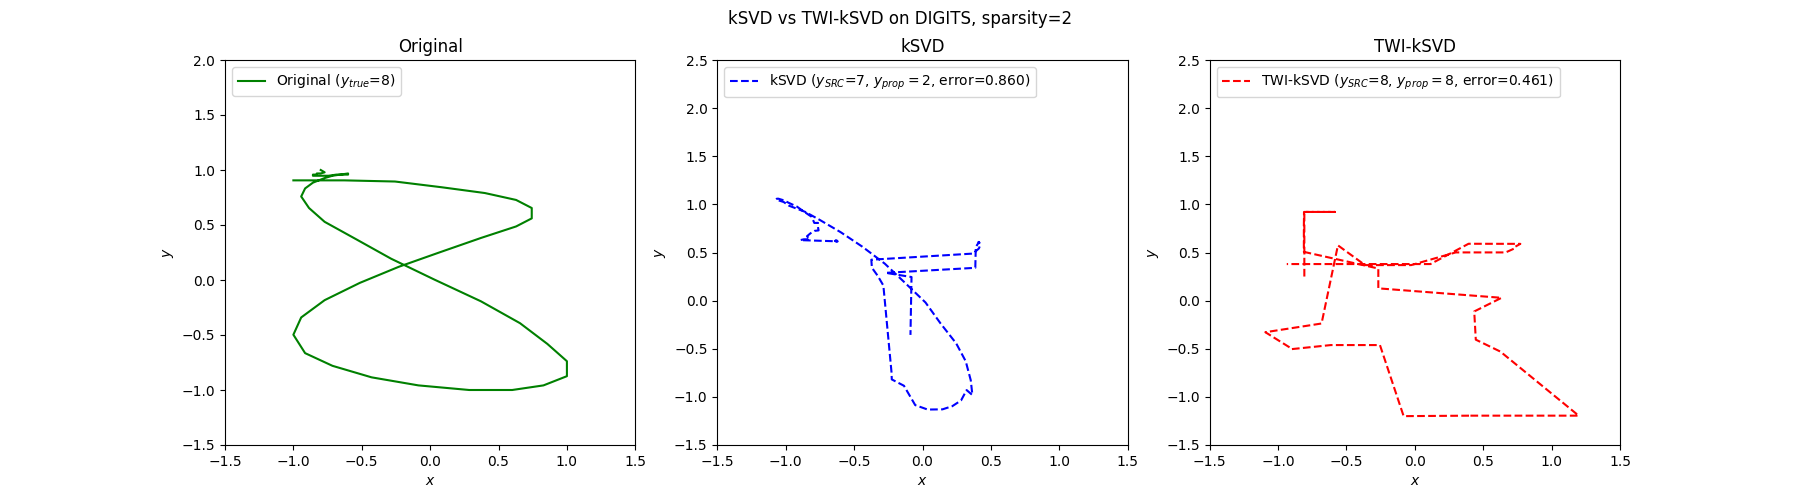
\includegraphics[width=\textwidth]{../../figures/2D_example_sparsity_2.png}
        \caption{Sparsity = 2}
    \end{subfigure}
    
    \begin{subfigure}[t]{\textwidth}
        \centering
        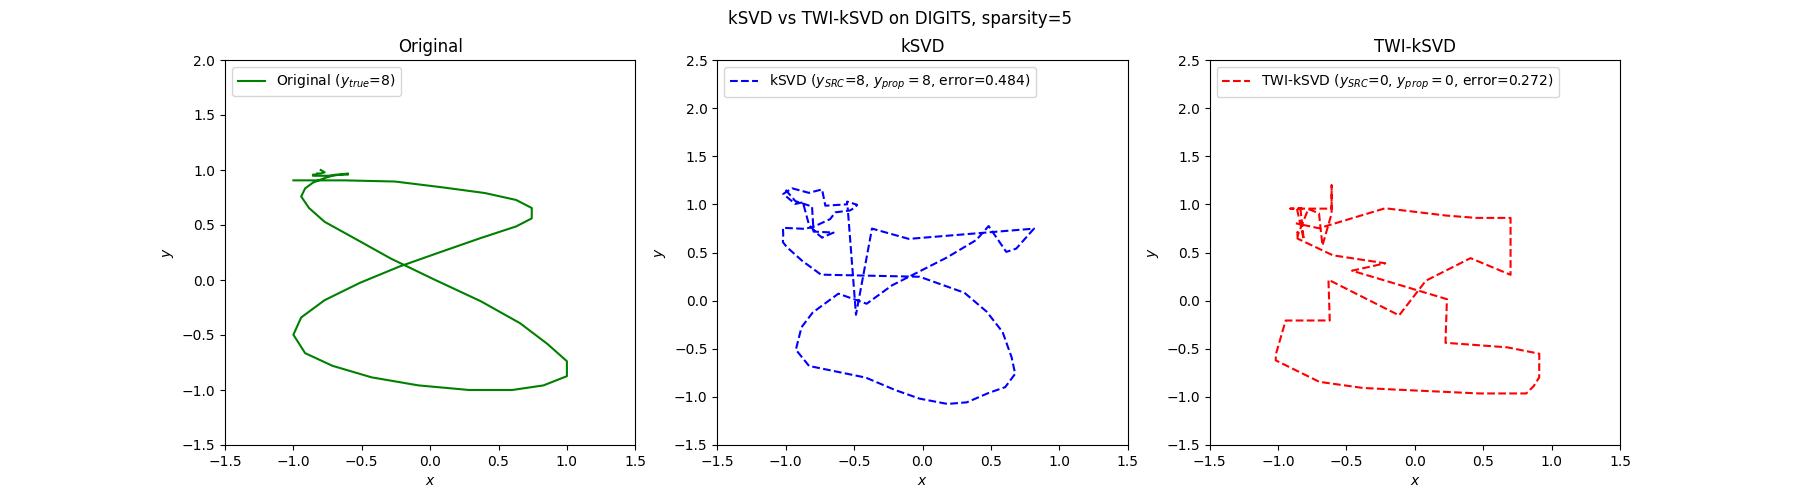
\includegraphics[width=\textwidth]{../../figures/2D_example_sparsity_5.png}
        \caption{Sparsity = 5}
    \end{subfigure}

    \begin{subfigure}[t]{\textwidth}
        \centering
        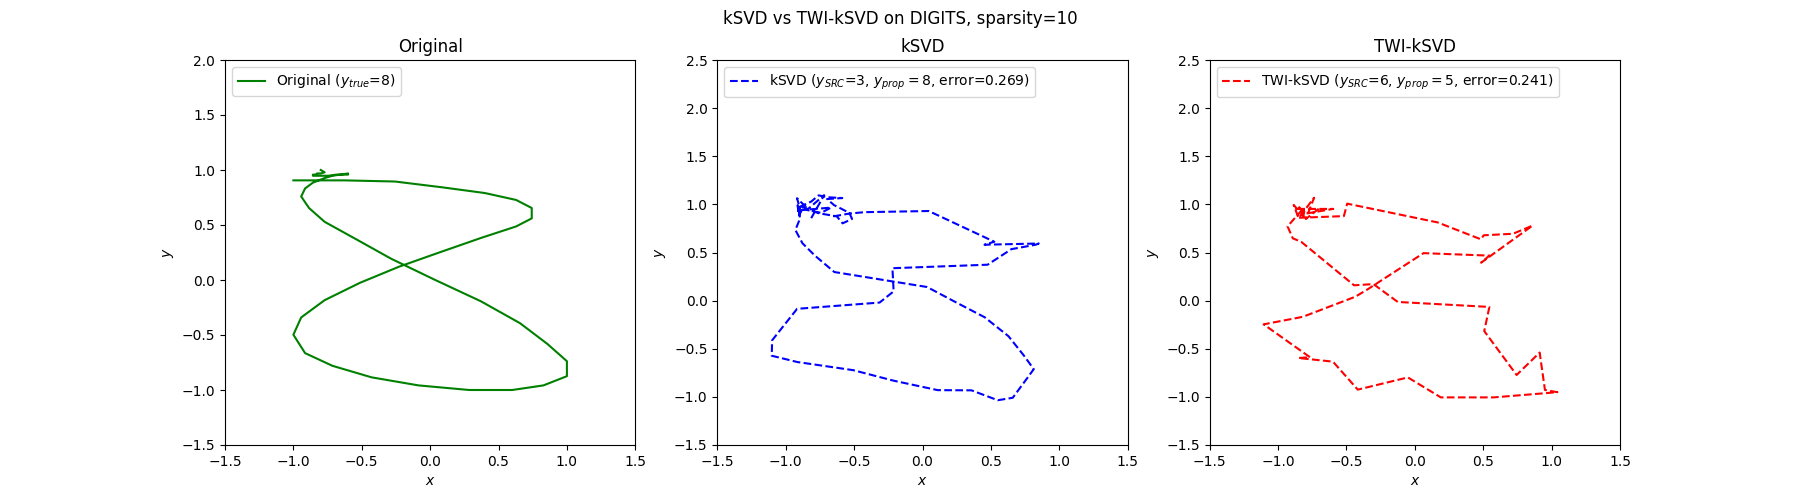
\includegraphics[width=\textwidth]{../../figures/2D_example_sparsity_10.png}
        \caption{Sparsity = 10}
    \end{subfigure}
        \caption{Example of reconstructions (DIGITS dataset) with different sparsity levels}\label{tab:2D_example}
\end{figure*}

%%%%%%%%% REFERENCES
{\small
\bibliographystyle{acm}
\bibliography{biblio}
}

\end{document}
